\section{Numerical results}\label{sec:numerics}

\begin{figure}[H]
    \centering
    \begin{subfigure}{0.32\textwidth}
        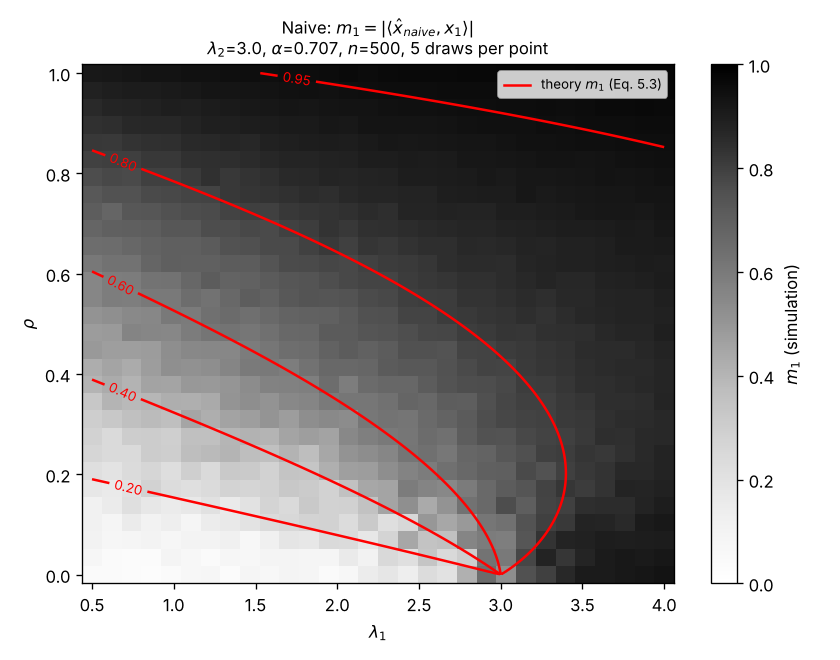
\includegraphics[width=\textwidth]{figures/heat_overlap_naive1_lam2=3.0_n=500.png}
        \caption{}
    \end{subfigure}\hfill
    \begin{subfigure}{0.32\textwidth}
        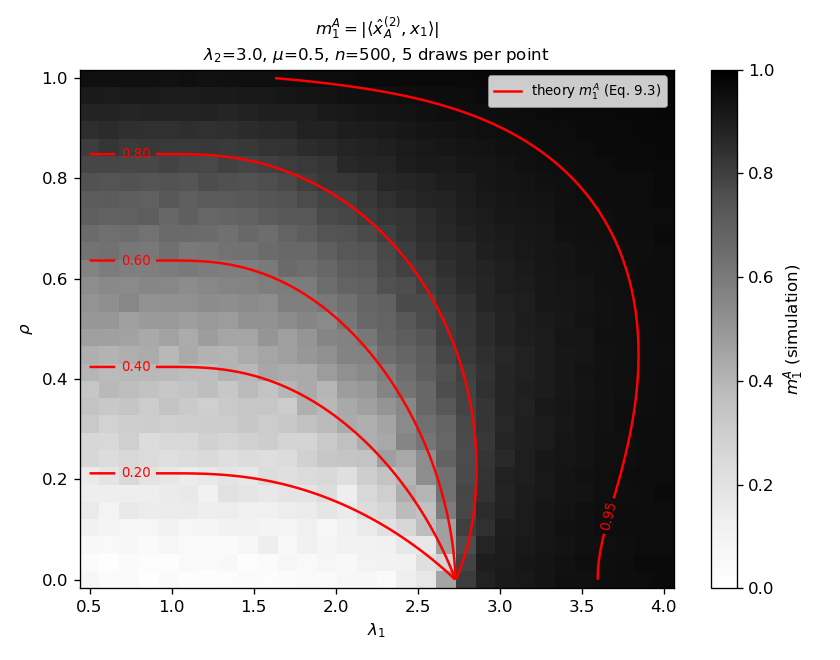
\includegraphics[width=\textwidth]{figures/heat_overlap_A_lam2=3.0_mu=0.5_n=500.png}
        \caption{}
    \end{subfigure}\hfill
    \begin{subfigure}{0.32\textwidth}
        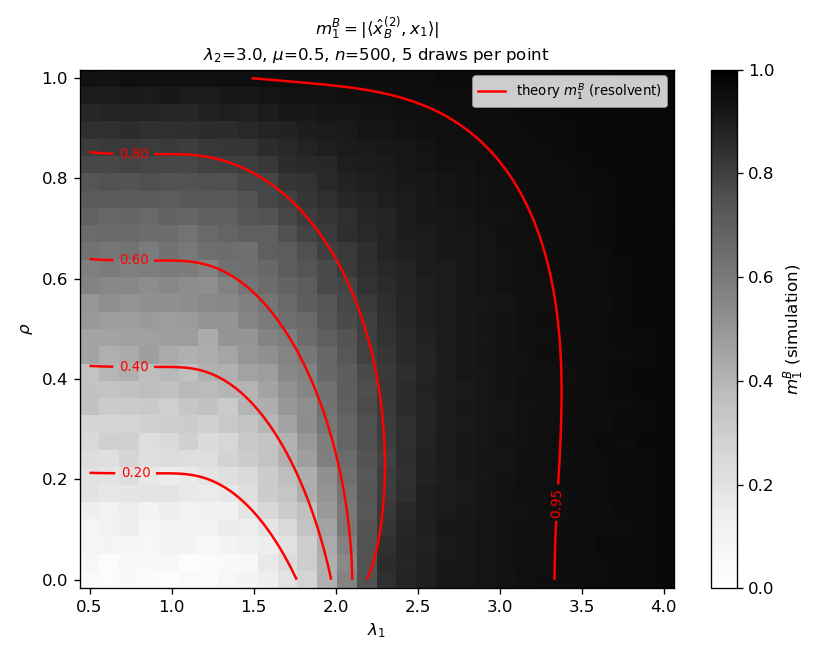
\includegraphics[width=\textwidth]{figures/heat_overlap_B1_lam2=3.0_mu=0.5_n=500.png}
        \caption{}
    \end{subfigure}
    \caption{}
    \label{fig:heat_overlap_1}
\end{figure}

\begin{figure}[H]
    \centering
    \begin{subfigure}{0.32\textwidth}
        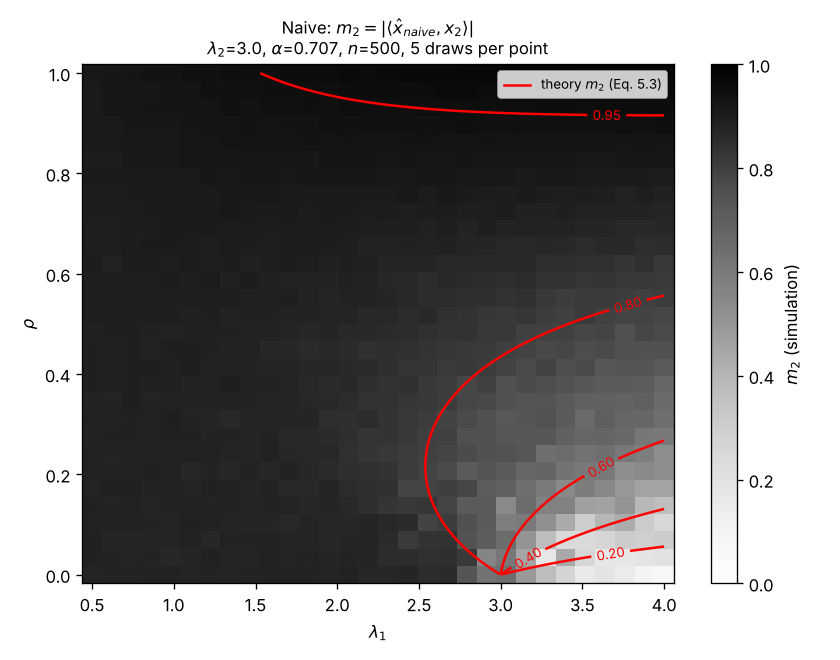
\includegraphics[width=\textwidth]{figures/heat_overlap_naive2_lam2=3.0_n=500.png}
        \caption{}
    \end{subfigure}\hfill
    \begin{subfigure}{0.32\textwidth}
        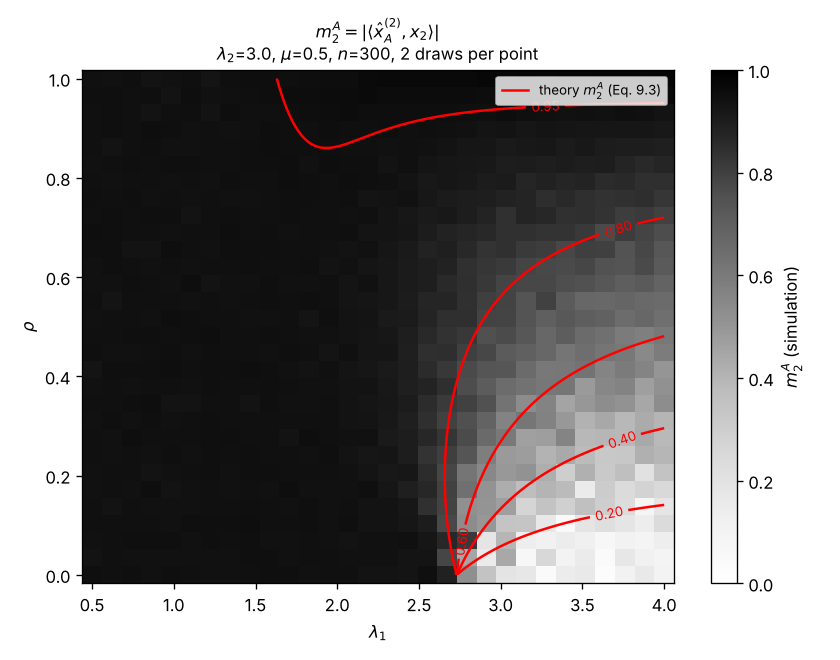
\includegraphics[width=\textwidth]{figures/heat_overlap_A2_lam2=3.0_mu=0.5_n=300.png}
        \caption{}
    \end{subfigure}\hfill
    \begin{subfigure}{0.32\textwidth}
        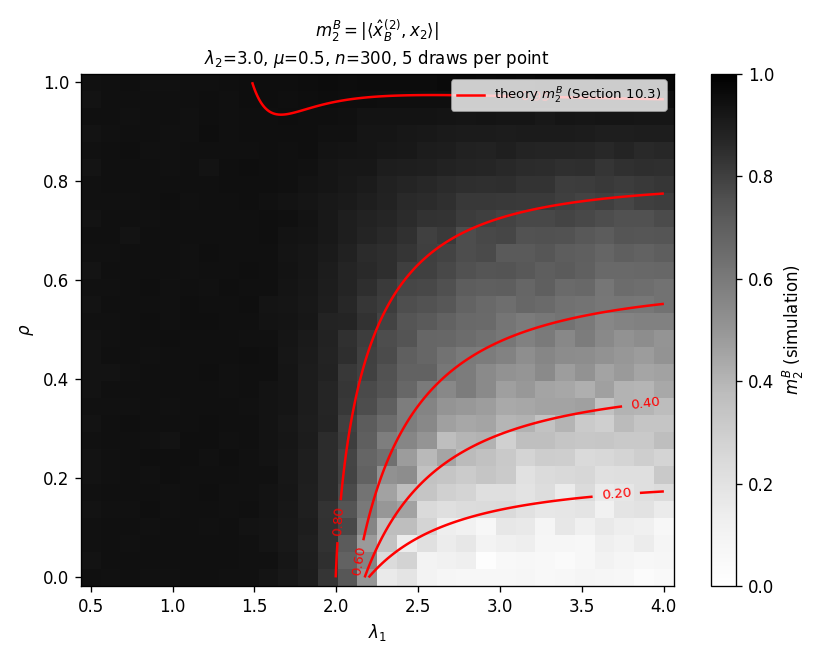
\includegraphics[width=\textwidth]{figures/heat_overlap_B2_lam2=3.0_mu=0.5_n=300.png}
        \caption{}
    \end{subfigure}
    \caption{}
    \label{fig:heat_overlap_2}
\end{figure}

\begin{figure}[H]
    \centering
    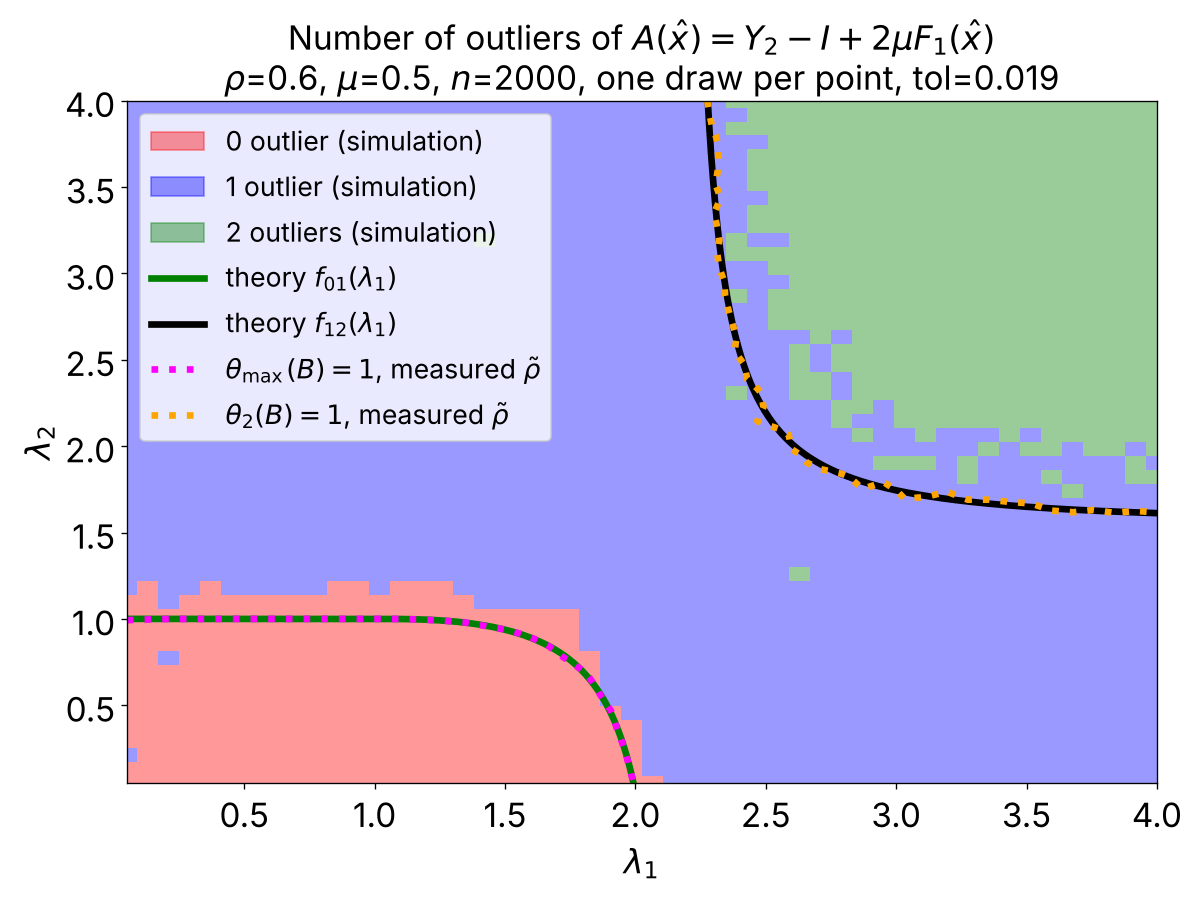
\includegraphics[width=0.5\linewidth]{figures/phase_A_rho=0.6_n=2000_fullB.png}
    \caption{}
    \label{fig:phase_A_outliers}
\end{figure}

\begin{figure}[H]
    \centering
    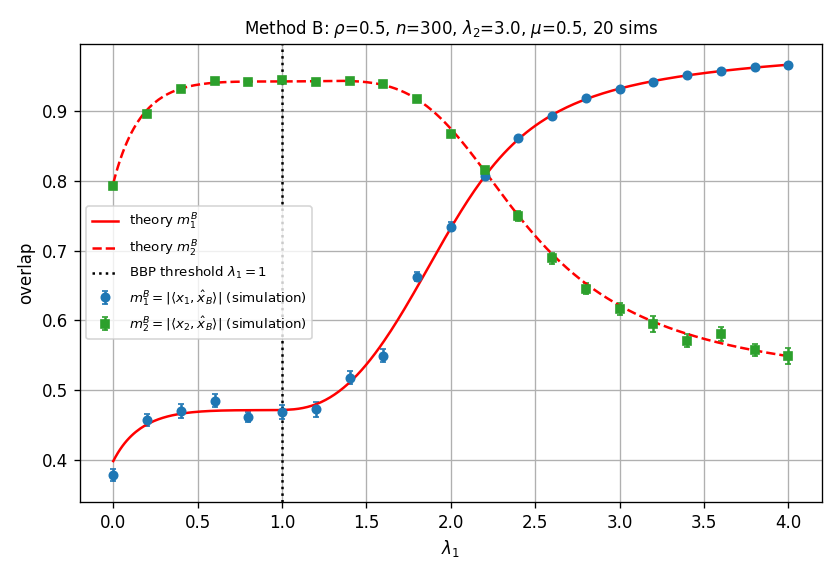
\includegraphics[width=0.5\linewidth]{figures/overlap_B_vs_lam1_rho=0.5_n=300.png}
    \caption{}
    \label{fig:overlap_B_vs_lam1}
\end{figure}

\begin{figure}[H]
    \centering
    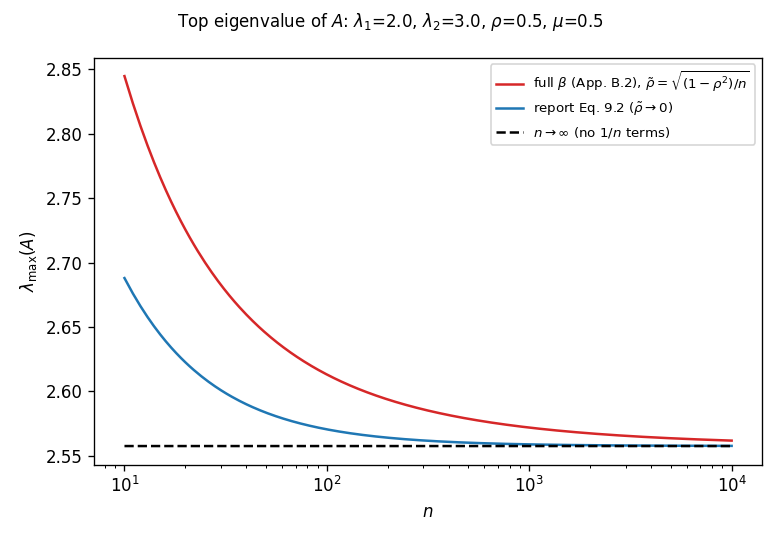
\includegraphics[width=0.5\linewidth]{figures/top_eig_A_old_vs_new_lam1=2.0_lam2=3.0_rho=0.5_mu=0.5.png}
    \caption{}
    \label{fig:top_eig_A}
\end{figure}

\begin{figure}[H]
    \centering
    \begin{subfigure}{0.32\textwidth}
        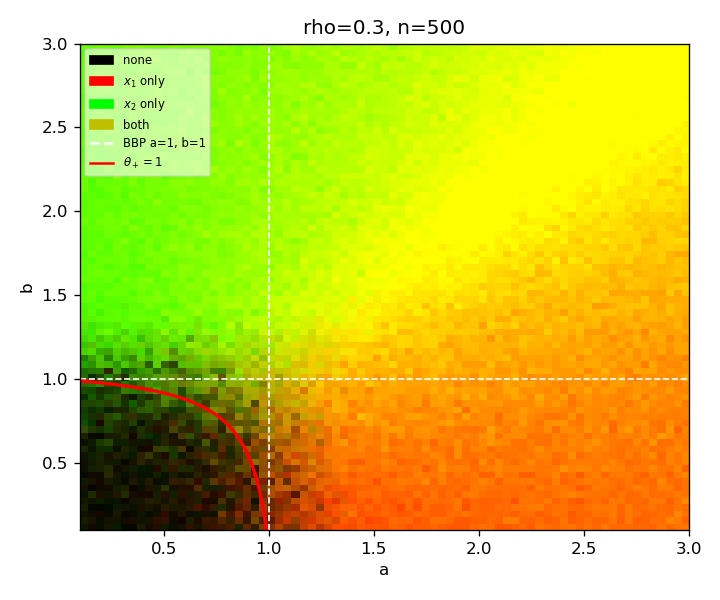
\includegraphics[width=\textwidth]{figures/phase_rho=0.3.png}
        \caption{}
    \end{subfigure}\hfill
    \begin{subfigure}{0.32\textwidth}
        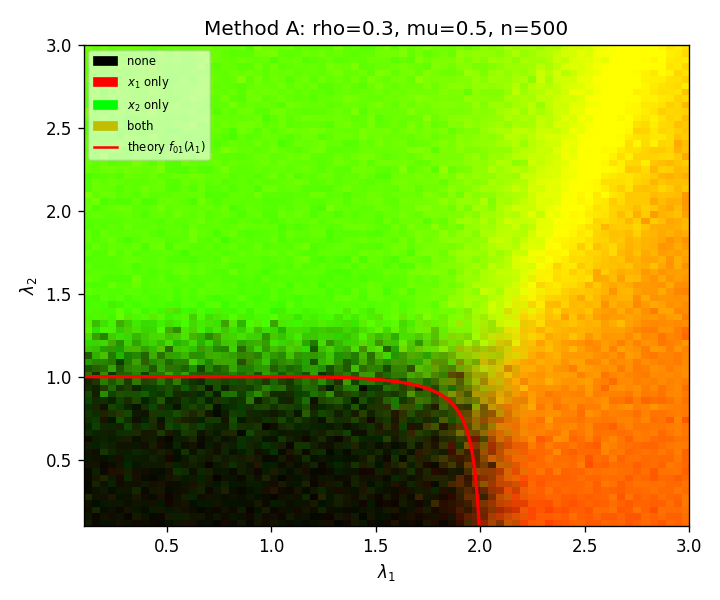
\includegraphics[width=\textwidth]{figures/phase_method_A_rho=0.3_n=500_reps=3.png}
        \caption{}
    \end{subfigure}\hfill
    \begin{subfigure}{0.32\textwidth}
        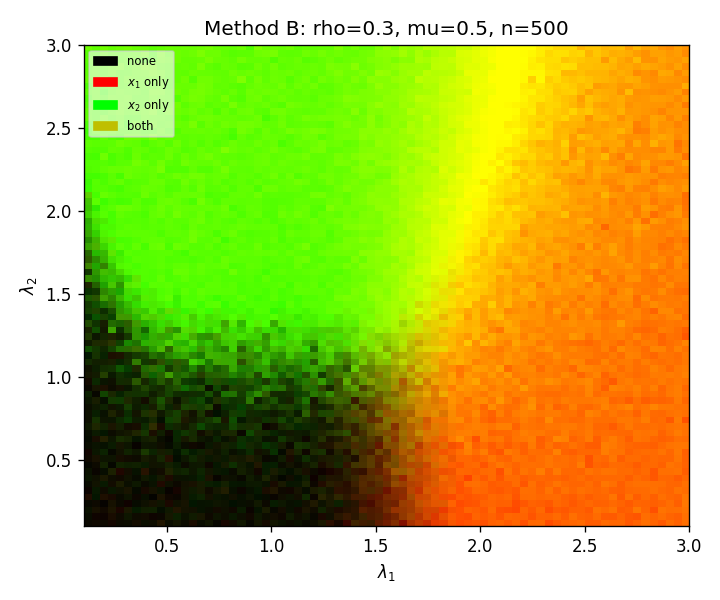
\includegraphics[width=\textwidth]{figures/phase_method_B_rho=0.3_n=500_reps=3.png}
        \caption{}
    \end{subfigure}
    \caption{}
    \label{fig:phase_rho_0_3}
\end{figure}

